% ============================================================
%  Exercise 5 Redone -- CMOS Inverter Chain Delay Optimisation
%  2-page landscape handout, 4 slide boxes per page
%
%  HOW TO COMPILE ON OVERLEAF:
%  Upload this file plus the following images (rename as shown):
%    case1_single_rg0.png          <- With_1pF_load/images/case1_single_rg0.png
%    case2_single_rg1.png          <- With_1pF_load/images/case2_single_rg1.png
%    case3_m_based.png             <- With_1pF_load/images/case3_m_based.png
%    case4_nf_finger.png           <- With_1pF_load/images/case4_nf_finger.png
%    delay_comparison_c1_c3_c4.png <- With_1pF_load/images/delay_comparison_c1_c3_c4.png
%    delay_10pF.png                <- With_10pF_load/delay_10pF.png
% ============================================================
\documentclass[a4paper,landscape,11pt]{article}
\usepackage[utf8]{inputenc}
\usepackage{graphicx}
\usepackage{amsmath}
\usepackage{geometry}
\usepackage{tikz}
\usepackage{booktabs}
\usepackage{helvet}
\usepackage[colorlinks=true, urlcolor=blue]{hyperref}

\renewcommand{\familydefault}{\sfdefault}

\geometry{margin=1cm}

% Set graphicspath so images can be found in their original folders
\graphicspath{{SPECTRE/EXERCISE5/With_1pF_load/images/}{SPECTRE/EXERCISE5/With_10pF_load/}}

% Slide box: fixed 13.5cm x 8.5cm, content clipped to fit
\newcommand{\slidebox}[2]{%
    \begin{tikzpicture}
        \draw[thick] (0,0) rectangle (13.5, 8.5);
        \node[anchor=north west, inner sep=0pt, yshift=-5pt] at (0,0) {\footnotesize #1};
        \clip (0.1,0.1) rectangle (13.4,8.4);
        \node[anchor=center] at (6.75, 4.25) {
            \begin{minipage}{12.5cm}
                #2
            \end{minipage}
        };
    \end{tikzpicture}%
}

\begin{document}
\pagestyle{empty}

% ==================== PAGE 1 ====================
\noindent
\slidebox{1}{} % Empty -- professor notes
\hfill
\slidebox{2}{} % Empty -- professor notes

\vspace{0.5cm}

\noindent
\slidebox{3}{} % Empty -- professor notes
\hfill
\slidebox{4}{
    \vspace{1.5cm}
    \hspace{1cm}
    \begin{tabular}{l}
        \LARGE \textbf{Exercise 5 Redone} \\[0.3em]
        \vspace{0.4cm}
\scriptsize \href{https://drive.google.com/file/d/1HsAws_kU7poEELz8WfXPL0r3M5Wf-Fd4/view?usp=sharing}{View Back-of-the-Envelope Calculations (PDF)}

    \end{tabular}
}

\newpage
% ==================== PAGE 2 ====================

% ---- Box 5 : Case 1 vs Case 2  (1 pF, single device, rgatemod 0 vs 1) ----
\noindent
\slidebox{5}{
    \centering
    \textbf{Case 1 vs.\ Case 2 \textemdash{} Single Wide Device, $C_L = 1\,$pF}\\[0.15cm]
    \begin{minipage}[t]{5.2cm}
        \centering
        {\scriptsize \textbf{Case 1:} \texttt{rgatemod = 0} (gate $R$ disabled)}\\[0.02cm]
        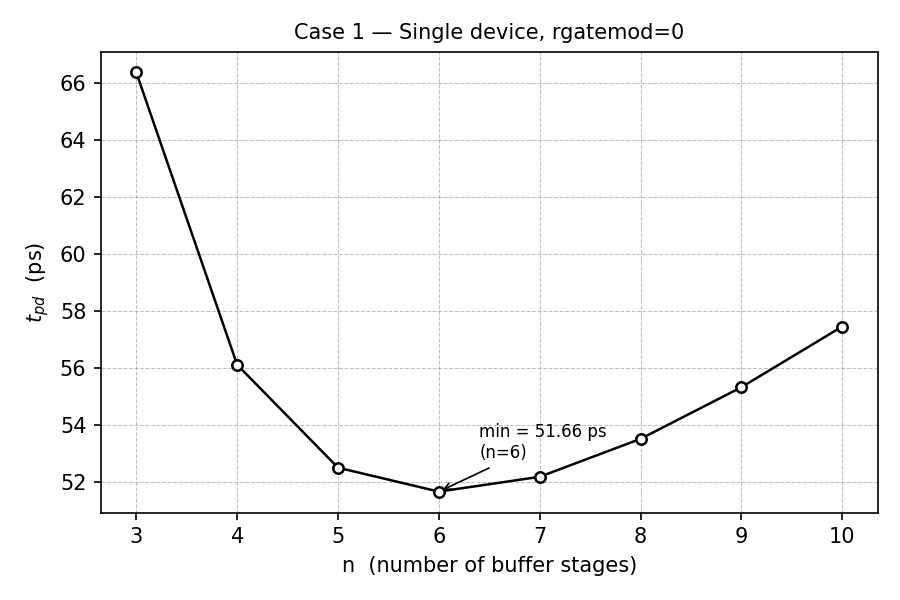
\includegraphics[width=5.0cm,height=3.4cm,keepaspectratio]{case1_single_rg0.png}
    \end{minipage}%
    \hfill
    \begin{minipage}[t]{5.2cm}
        \centering
        {\scriptsize \textbf{Case 2:} \texttt{rgatemod = 1} (gate $R$ enabled)}\\[0.02cm]
        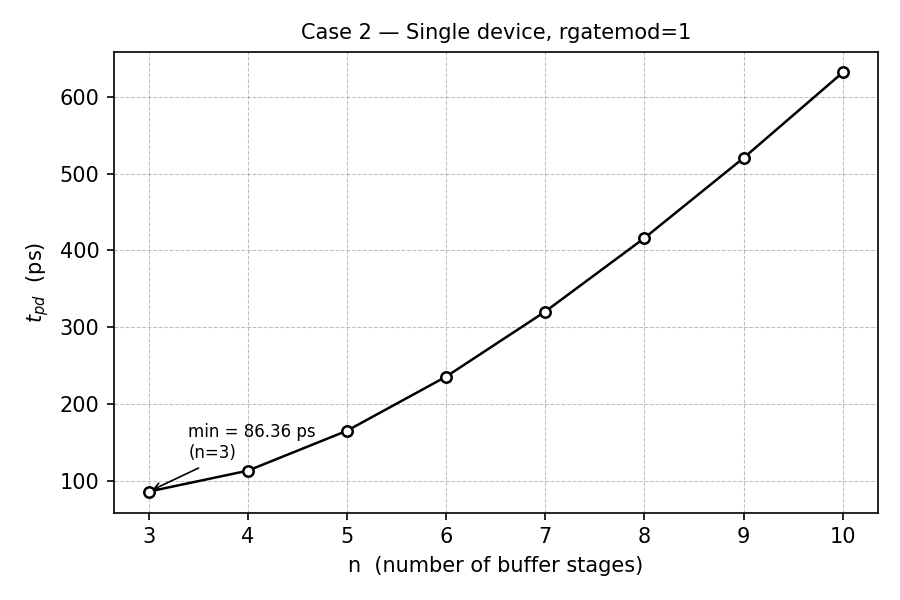
\includegraphics[width=5.0cm,height=3.4cm,keepaspectratio]{case2_single_rg1.png}
    \end{minipage}\\[0.05cm]
    \scriptsize
    \begin{tabular}{@{}lcc@{}}
        \toprule
        & \textbf{Case 1} & \textbf{Case 2} \\
        \midrule
        \texttt{rgatemod}    & 0              & 1 \\
        Min $t_{pd}$         & \textbf{51.66\,ps} & 86.36\,ps \\
        Optimal $n$          & 6              & 3 (sweep lower bound) \\
        Delay trend          & Convex, clear min.\ & Monotonically rising \\
        \bottomrule
    \end{tabular}\\[0.1cm]
   
}
\hfill
% ---- Box 6 : Case 3 vs Case 4  (1 pF, m-based vs nf multi-finger) ----
\slidebox{6}{
    \centering
    \textbf{Case 3 vs.\ Case 4 \textemdash{} Gate-$R$ Aware Methods, $C_L = 1\,$pF}\\[0.15cm]
    \begin{minipage}[t]{5.2cm}
        \centering
        {\scriptsize \textbf{Case 3:} \texttt{m}-based parallel (\texttt{rgatemod=1})}\\[0.02cm]
        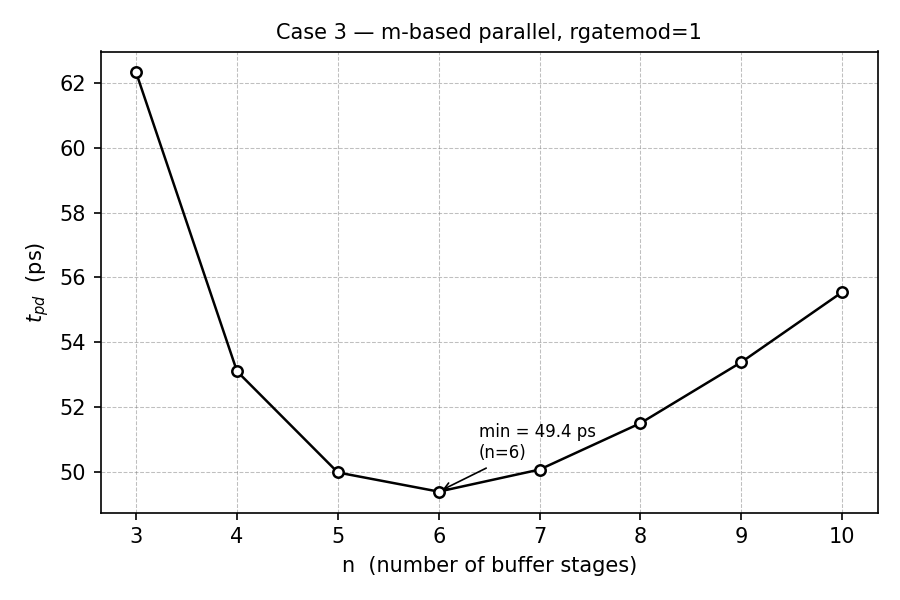
\includegraphics[width=5.0cm,height=3.4cm,keepaspectratio]{case3_m_based.png}
    \end{minipage}%
    \hfill
    \begin{minipage}[t]{5.2cm}
        \centering
        {\scriptsize \textbf{Case 4:} \texttt{nf} fingers $W_f\!=\!220\,$nm (\texttt{rgatemod=1})}\\[0.02cm]
        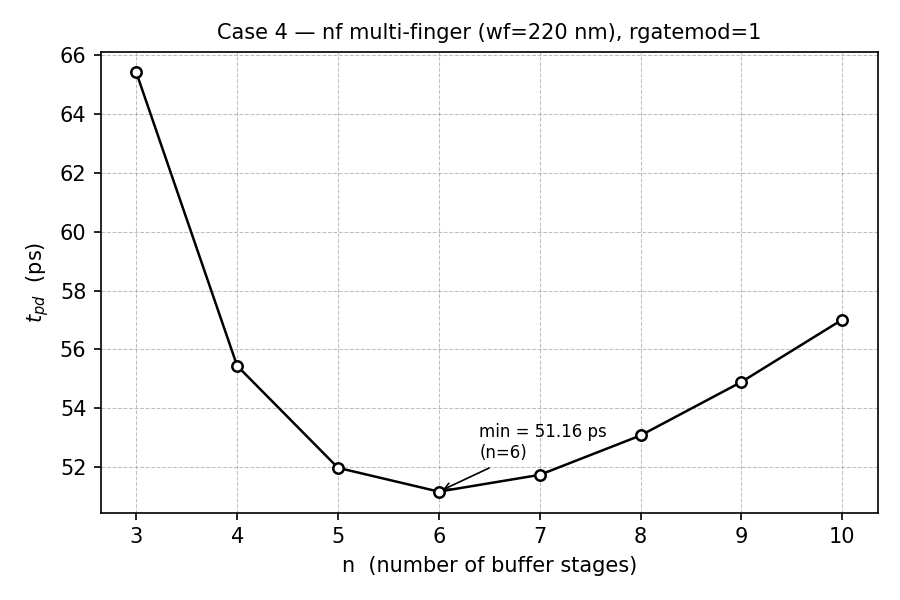
\includegraphics[width=5.0cm,height=3.4cm,keepaspectratio]{case4_nf_finger.png}
    \end{minipage}\\[0.05cm]
    \scriptsize
    \begin{tabular}{@{}lcc@{}}
        \toprule
        & \textbf{Case 3} & \textbf{Case 4} \\
        \midrule
        Scaling          & \texttt{m} multiplicity   & $NF=\lceil W_{tot}/W_f\rceil$ \\
        Min $t_{pd}$     & \textbf{49.40\,ps}        & 51.16\,ps \\
        Optimal $n$      & 6                          & 6 \\
        Setup effort     & Lower                        & High \\
        Layout fidelity  & Medium                     & \textbf{High} \\
        \bottomrule
    \end{tabular}\\[0.1cm]
    
}

\vspace{0.5cm}

\noindent
% ---- Box 7 : Comparison plot Cases 1, 3, 4  (1 pF) ----
\slidebox{7}{
    \centering
    \textbf{Comparative Analysis \textemdash{} Cases 1, 3 \& 4\quad($C_L = 1\,$pF)}\\[0.02cm]
    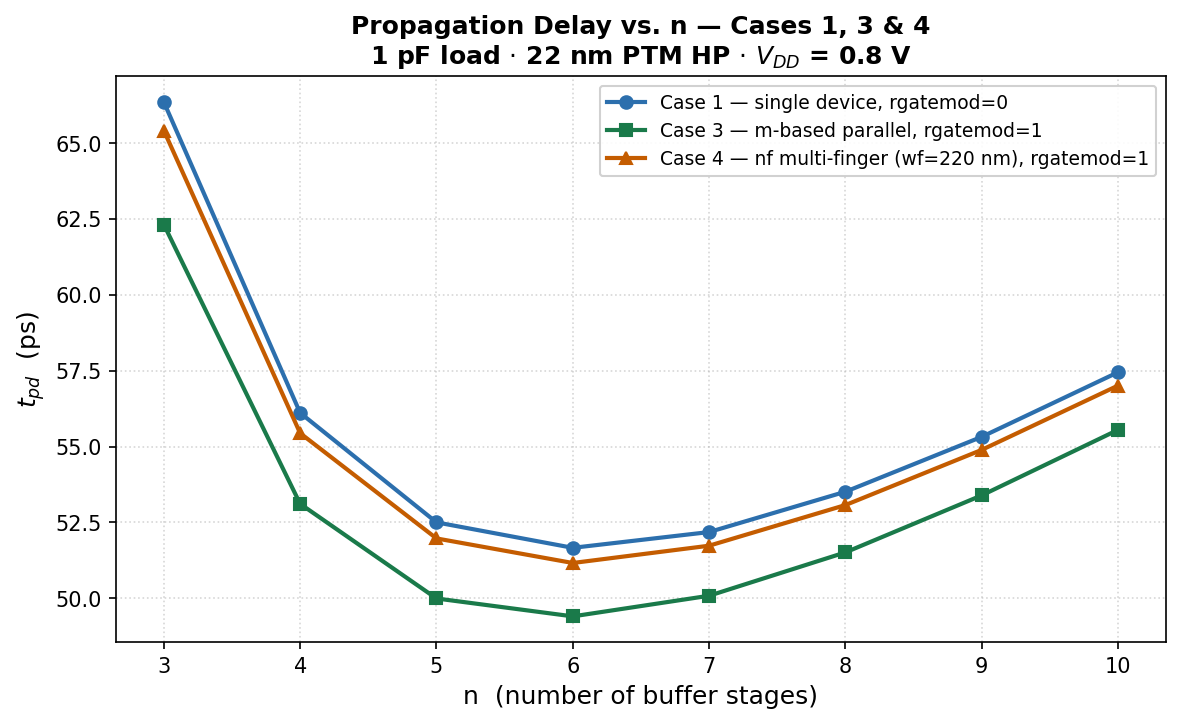
\includegraphics[width=10.5cm,height=4.5cm,keepaspectratio]{delay_comparison_c1_c3_c4.png}\\[0.05cm]
    \scriptsize
    \begin{tabular}{@{}lccc@{}}
        \toprule
        & \textbf{Case 1} & \textbf{Case 3} & \textbf{Case 4} \\
        \midrule
        Setup effort  & \textbf{Easiest} (scale \texttt{w})
                      & Medium (\texttt{m} param)
                      & Most ($NF$ per stage) \\
        Accuracy      & \textbf{Least} (\texttt{rgatemod=0})
                      & More
                      & \textbf{Most} (layout-rep.) \\
        Min $t_{pd}$  & 51.66\,ps & \textbf{49.40\,ps} & 51.16\,ps \\
        Optimal $n$   & 6 & 6 & 6 \\
        \bottomrule
    \end{tabular}
}
\hfill
% ---- Box 8 : 10 pF result ----
\slidebox{8}{
    \centering
    \textbf{\texttt{nf} Multi-finger Method \textemdash{} $C_L = 10\,$pF}\\[0.02cm]
    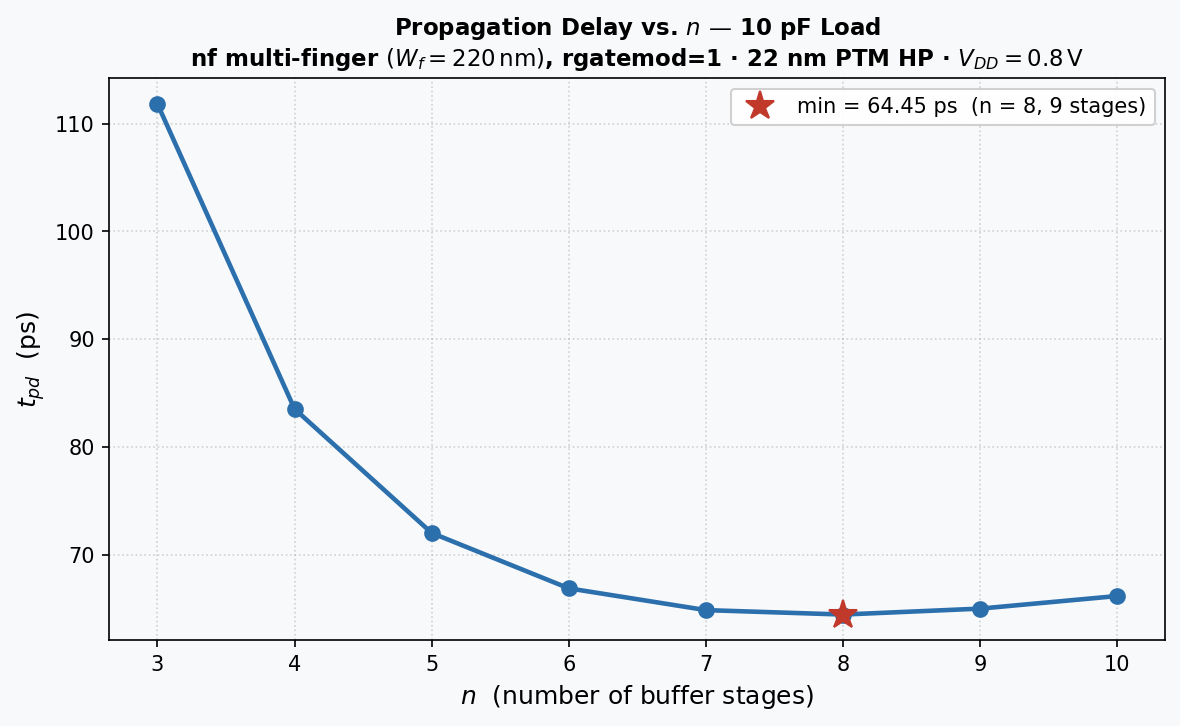
\includegraphics[width=10.0cm,height=4.2cm,keepaspectratio]{delay_10pF.png}\\[0.02cm]
    \scriptsize
    \begin{tabular}{@{}lcc@{}}
        \toprule
        & $C_L = 1\,$pF & $C_L = 10\,$pF \\
        \midrule
        $M = C_L/C_{in}$   & 13\,661   & 136\,612 \\
        Optimal $n$         & 6         & \textbf{8} \\
        Optimal stages      & 7         & \textbf{9} \\
        Min $t_{pd}$        & 51.16\,ps & \textbf{64.45\,ps} \\
        Optimal $\alpha$    & 3.897     & \textbf{3.721} \\
        \bottomrule
    \end{tabular}\\[0.06cm]
    
}

\end{document}
